\documentclass[a4paper]{article}
\usepackage[a4paper,top=1cm,bottom=1.5cm,left=1.5cm,right=1.5cm,marginparwidth=1cm]{geometry}
%% Language and font encodings
\usepackage[german]{babel}
\usepackage[utf8x]{inputenc}
\usepackage{listings}
\usepackage{caption}
\usepackage{subcaption}

%% Sets page size and margins

\usepackage{float}
%% Useful packages
\usepackage{amsmath}
\usepackage[colorinlistoftodos]{todonotes}
\usepackage[colorlinks=true, allcolors=blue]{hyperref}
\usepackage{listings}
\usepackage{url}
\usepackage{graphicx}
\graphicspath{ {./images/} }
% \DeclareGraphicsExtensions{.pdf,.jpg,.png}

%% defined colors
\definecolor{Blue}{rgb}{0,0,0.5}
\definecolor{Green}{rgb}{0,0.75,0.0}
\definecolor{LightGray}{rgb}{0.6,0.6,0.6}
\definecolor{DarkGray}{rgb}{0.3,0.3,0.3}
\setlength{\parindent}{0pt}

\title{AVIS Einführungsaufgabe - Performanz-Messung}
\author{
Martin ben Ahmed (970697) \\ 
}
\date{\today}
 

\begin{document}
\maketitle

\section*{Durchsatzmessung über zunehmende Distanzen}
\noindent
\begin{figure}[ht]
  \centering
  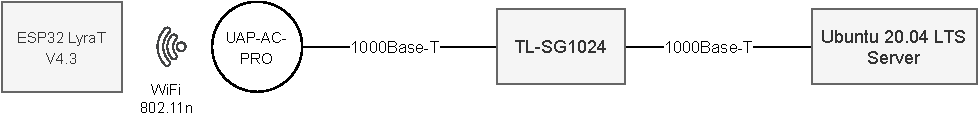
\includegraphics[width=.6\linewidth]{../images/network_architecture.pdf} 
  \caption{Versuchsaufbau.}
  \label{fig:net_arch}
\end{figure}

Mithilfe des Tools \emph{iperf} wurde der Durchsatz zwischen LyraT Board und Server gemessen.
Der Versuchsaufbau besteht aus den folgenden Hardwarekomponenten:
\begin{itemize}
  \item Espressif ESP32-LyraT Board
  \item Ubiquiti UniFi UAP-AC-PRO Access Point 
  \item TP-Link TL-SG1024 Unmanaged Switch
  \item Ubuntu 20.04 LTS Server (i5 3570k, 16 GB DDR3)
\end{itemize}

Das LyraT Board ist per WiFi (802.11n) mit dem Access Point verbunden. 
Der Access Point ist per Gigabit Ethernet mit dem Switch verbunden.
Switch und Server sind ebenfalls per Gigabit Ethernet mit einander verbunden.
Für die Messung wurde der Switch vom restlichen Netz getrennt.
Der Versuchsaufbau ist in Abbildung~\ref{fig:net_arch} dargestellt.

Der Durchsatz zwischen LyraT Board und Server wurde in mbit/s gemessen. 
Der Abstand zwischen Access Point und Board wurde dabei in 15 Meter Schritten sukzessive vergrößert.
Es wurden sowohl TCP als auch UDP gemessen. 
Die Messung mit 0 Meter Abstand wurde innerhalb eines Wohnhauses durchgeführt.
Alle weiteren Messungen fanden außerhalb des Hauses statt, wodurch sich eine Dämpfung des Signals aufgrund der Wände und Decken ergibt.
Außerhalb des Hauses befanden sich keine weiteren Hindernisse zwischen LyraT Board und Access Point.

\begin{figure}[ht]
  \begin{subfigure}{.5\textwidth}
    \centering
    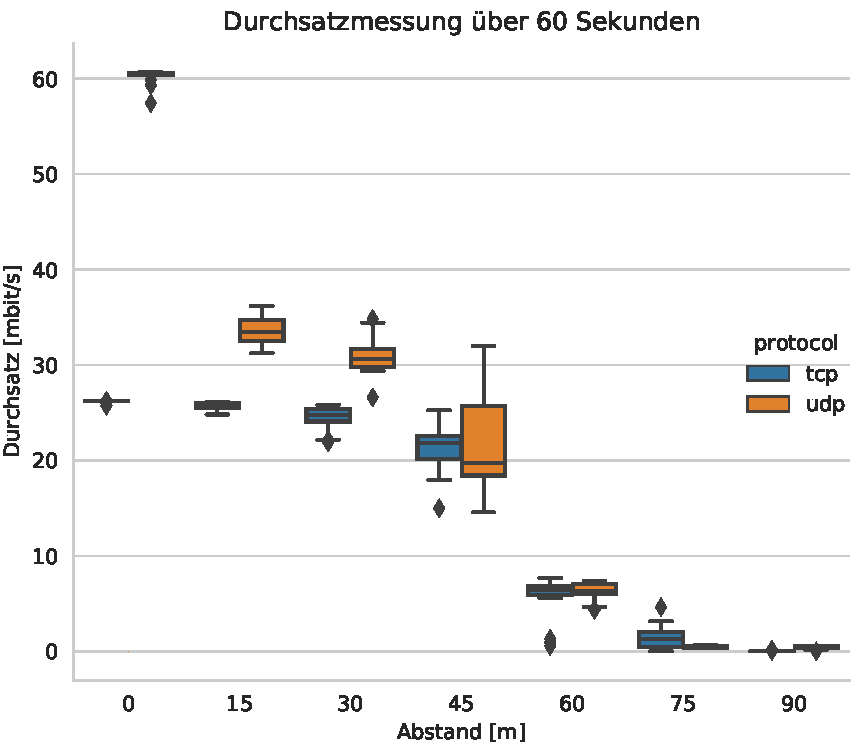
\includegraphics[width=.9\linewidth]{../images/box.pdf} 
    \caption{Verteilung des Durchsatzes pro Abstand.}
    \label{fig:box}
  \end{subfigure}
  \begin{subfigure}{.5\textwidth}
    \centering
    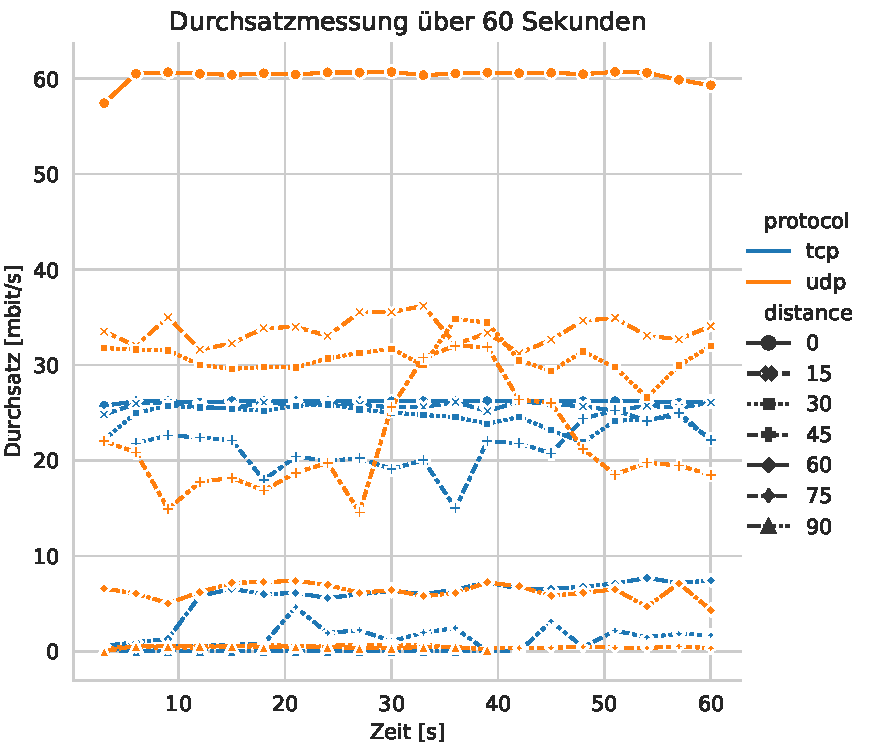
\includegraphics[width=.9\linewidth]{../images/line.pdf} 
    \caption{Zeitlicher Verlauf des Durchsatzes.}
    \label{fig:line}
  \end{subfigure}
  \caption{Durchsatzmessung über 60 Sekunden.}
  \label{fig:performance}
\end{figure} 

  Die Messungen haben ergeben, dass die technische Obergrenze von TCP bei etwa 26 mbit/s liegt und von UDP bei etwa 60 mbit/s. 
  Wie in Abbildung~\ref{fig:box} zu erkennen, bricht die Durchsatzrate erst ab etwa 60 Meter Abstand deutlich ein. 
  Da der Durchsatz von TCP durch andere Faktoren beschränkt wird, wirkt sich die Signalstärke erst ab 45 Meter Abstand auf den Durchsatz aus. 
  UDP erzielt näher am Access Point deutlich höhere Datenraten als TCP. 
  Bei der Messung mit 45 m Abstand traten sowohl bei UDP als auch TCP die größten Abweichungen auf (Abb.~\ref{fig:line}).
  Alle übrigen Messungen ergaben eine relativ konstante Durchsatzrate.  
\end{document}